\documentclass[a4paper, 10pt]{article}
% (1) Encoding, Fonts, and Layout
\usepackage[T1]{fontenc}
\usepackage{lmodern}
\usepackage[margin=1in]{geometry}


% (2) Common Packages
\usepackage{amsmath, amssymb, amsthm}
\usepackage{xcolor}
\usepackage{caption}
\usepackage{tikz}
\usepackage{pgfplots}
\pgfplotsset{compat=newest}
\usepackage{etoolbox}
\usepackage{tikz-3dplot}
\tdplotsetmaincoords{75}{120}
\usepackage[inline]{enumitem}
\usepackage{bookmark}
\usepackage{mathtools}
\usepackage{subcaption} % For subfigures
\usepackage[normalem]{ulem} % For better underline commands

% Micro-typography
\usepackage{microtype}

% Patching pgfplots warning
\makeatletter
\patchcmd{\pgfplots@applistXXpushback@smallbuf}{\pgfplots@error}{\pgfplots@warning}{}{}
\makeatother

% (3) tcolorbox and Theorem Libraries
\usepackage{tcolorbox}
\tcbuselibrary{theorems}

% (4) Define Colors
\definecolor{custom_green}{HTML}{a3be8c}
\definecolor{custom_red}{HTML}{dc322f}
\definecolor{custom_blue}{HTML}{268bd2}
\definecolor{custom_purple}{HTML}{b48ead}

\definecolor{base}{HTML}{eceff4}
\definecolor{gray1}{HTML}{e5e9f0}
\definecolor{gray2}{HTML}{d8dee9}
\definecolor{gray3}{HTML}{2e3440}
\pagecolor{base}

% (5) Custom tcolorbox Environments
\newtcolorbox{definitionbox}[1][]{
    title=\textbf{Definition} {#1},
    fonttitle=\bfseries\boldmath,
    arc=0mm,
    bottomtitle=0.5mm,
    boxrule=0mm,
    colbacktitle=gray2,
    colback=gray1,
    coltitle=gray3,
    coltext=gray3,
    left=2.5mm,
    leftrule=1mm,
    rightrule=1mm,
    right=3.5mm,
    toptitle=0.75mm,
    colframe=custom_red,
}

\newtcolorbox{proofbox}{
    title=\textbf{Proof},
    fonttitle=\bfseries\boldmath,
    arc=0mm,
    bottomtitle=0.5mm,
    boxrule=0mm,
    colbacktitle=gray2,
    colback=gray1,
    coltitle=gray3,
    left=2.5mm,
    leftrule=1mm,
    rightrule=1mm,
    right=3.5mm,
    toptitle=0.75mm,
    colframe=custom_blue,
    coltext=gray3,
}

\newtcolorbox{theorembox}[1][]{
    title=\textbf{Theorem} {#1},
    fonttitle=\bfseries\boldmath,
    arc=0mm,
    bottomtitle=0.5mm,
    boxrule=0mm,
    colbacktitle=gray2,
    colback=gray1,
    coltitle=gray3,
    left=2.5mm,
    leftrule=1mm,
    rightrule=1mm,
    right=3.5mm,
    toptitle=0.75mm,
    colframe=custom_green,
    coltext=gray3
}

\newtcolorbox{notebox}{
    title=\textbf{Note},
    fonttitle=\bfseries\boldmath,
    arc=0mm,
    bottomtitle=0.5mm,
    boxrule=0mm,
    colbacktitle=gray2,
    coltitle=gray3,
    left=2.5mm,
    leftrule=1mm,
    rightrule=1mm,
    right=3.5mm,
    toptitle=0.75mm,
    colframe=custom_blue,
    coltext=gray3
}

\newtcolorbox{examplebox}[1][]{
    title=\textbf{Example} {#1},
    fonttitle=\bfseries\boldmath,
    arc=0mm,
    bottomtitle=0.5mm,
    boxrule=0mm,
    colbacktitle=gray2,
    colback=gray1,
    coltitle=gray3,
    left=2.5mm,
    leftrule=1mm,
    rightrule=1mm,
    right=3.5mm,
    toptitle=0.75mm,
    colframe=gray3,
    fontupper=\footnotesize,
    coltext=gray3
}

% (6) Theorem Environments
\theoremstyle{definition}
\newtheorem{definition}{Definition}[section]
\newtheorem{example}[definition]{Example}

\theoremstyle{plain}
\newtheorem{theorem}[definition]{Theorem}

% (7) Hyperlinks
\usepackage{hyperref}
\hypersetup{
    colorlinks=true,    % Use colored text for links
    linkcolor=custom_red,      % Set link text color to red
    pdfborder={0 0 0}   % Remove the default box around links
}

% macros.tex
\newcommand{\intinf}{\int_0^{\infty}} % Integral from 0 to infinity
\newcommand{\diff}[2]{\frac{d#1}{d#2}} % Derivative



% Title and author
\title{
Robert Davidson \\
\textbf{MP232: Applied Mathematics}
}
\author{
60\% Exam\\
40\% Continuous Assessment (3 parts)
}
\date{} % Empty date

\begin{document}
\maketitle

\tableofcontents

\pagebreak
\section{Prelim : The Exponential Function and Hyperbolic Functions}
\subsection{Exponential Function}
\noindent \begin{minipage}{0.45\textwidth}
  \textbf{Derivative}
  $$\frac{d}{dt}\bigl(e^{at}\bigr) = a\,e^{at}$$
\end{minipage}\hfill
\noindent \begin{minipage}{0.45\textwidth}
  \textbf{Integral}
  $$\int e^{at}\,dt = \frac{1}{a}e^{at} + C$$
\end{minipage}\hfill



\subsection{Hyperbolic Functions}

\textbf{Definitions:}
$$
  \begin{array}{c | c | c}
    \sinh(at) = \frac{e^{at} - e^{-at}}{2}
     &
    \cosh(at) = \frac{e^{at} + e^{-at}}{2}
     &
    \tanh(at) = \frac{\sinh(at)}{\cosh(at)}.
  \end{array}
$$
\textbf{Derivatives}
$$
  \begin{array}{c | c | c}
    \frac{d}{dt}\bigl(\sinh(at)\bigr) = a\,\cosh(at),
     &
    \frac{d}{dt}\bigl(\cosh(at)\bigr) = a\,\sinh(at),
     &
    \frac{d}{dt}\bigl(\tanh(at)\bigr) = a\,\mathrm{sech}^2(at).
  \end{array}
$$
\textbf{Integrals}
\begin{align*}
  \int \sinh(at)\,dt & = \frac{1}{a}\cosh(at) + C                 \\
  \int \cosh(at)\,dt & = \frac{1}{a}\sinh(at) + C,                \\
  \int \tanh(at)\,dt & = \frac{1}{a}\ln\bigl|\cosh(at)\bigr| + C. \\
\end{align*}
\textbf{Common Identities}
\begin{align*}
  \cosh^2 x - \sinh^2 x & = 1,                                \\
  \sinh(2x)             & = 2\,\sinh x\,\cosh x,              \\
  \cosh(2x)             & = \cosh^2 x + \sinh^2 x,            \\
  \tanh(2x)             & = \frac{2\,\tanh x}{1 + \tanh^2 x}.
\end{align*}

\subsection{Partial Fraction Decomposition}
\textbf{Unrepeated Linear Factors}: A linear factor is of form $(ax + b)$
$$\frac{s + 1}{s(s-2)(s+3)} = \frac{A}{s} + \frac{B}{s-2} + \frac{C}{s+3}$$
\textbf{Repeated LinearFactors}:
$$\frac{3}{(s+2)^2(s-3)} = \frac{A}{s+2} + \frac{B}{(s+2)^2} + \frac{C}{s-3}$$
\textbf{Unrepeated Quadratic Factors with complex roots}: Where the discriminant ($b^2 - 4ac$) is \\
\indent negative (complex roots) but the factor is not repeated
$$\frac{3}{(s^2 - s + 1)(s+2)} = \frac{As + B}{s^2 - s + 1} + \frac{C}{s+2}$$
\textbf{Repeated Quadratic Factors with complex roots}:
$$\frac{1}{(s^2 + 1)^2 (s-1)} = \frac{As + B}{(s^2 + 1)^2} + \frac{Cs + D}{s^2 + 1} + \frac{E}{s-1}$$


\pagebreak
\section{Laplace Transforms}
\subsection{What is a Laplace Transform?}
The Laplace Transform, defined for $t \geq 0$, is given by
$$L\{f(t)\}(s) = F(s) = \int_0^\infty e^{-st} dt$$

\subsection{Common Laplace Transforms}

\begin{examplebox}[Find the Laplace Transform of \boldmath$f(t) = 1$]
  We have:
  $$L\{1\} = \int_0^\infty 1 \cdot e^{-st } dt = \lim_{R \to \infty} \int_0^R e^{-st} dt$$
  This integral is equal to:
  $$\int_0^R e^{-st} dt = \left . \frac{e^{-st}}{-s}\right |_{t=0}^{t=R}
    = -\frac{1}{s}[e^{-sR} - 1] = \frac{1 - e^{-sR}}{s}$$
  Taking the limit as $R \to \infty$ gives:
  $$L\{1\} = \lim_{R \to \infty} \frac{1 - e^{-sR}}{s} = \frac{1}{s}$$
\end{examplebox}

\begin{examplebox}[ Find the Laplace Transform of $f(t) = e^{2t}$]
  \begin{align*}
    L\{e^{2t}\}
     & = \int_0^\infty e^{2t}e^{-st}\, dt
    = \int_0^\infty e^{-(s-2)t}\, dt                                                                               \\[1mm]
     & = \lim_{R\to\infty} \int_0^R e^{-(s-2)t}\, dt                                                               \\[1mm]
     & = \lim_{R\to\infty} \left[ \frac{e^{-(s-2)t}}{-(s-2)} \right]_{t=0}^{t=R}                                   \\[1mm]
     & = \lim_{R\to\infty} \left( \frac{e^{-(s-2)R} - e^0}{-(s-2)} \right)
    = \lim_{R\to\infty} \left( \frac{e^{-(s-2)R} - 1}{-(s-2)} \right)                                              \\[1mm]
     & = \frac{1}{s-2} \quad \text{(since } e^{-(s-2)R} \to 0 \text{ as } R\to\infty \text{ provided } s>2\text{)}
  \end{align*}
\end{examplebox}

\begin{examplebox}[Find the Laplace Transform of $f(t) = \cosh(at)$]
  We have:
  \begin{align*}
    L\{\cosh(at)\} & = L\left\{ \frac{e^{at} + e^{-at}}{2}\right\} \quad \text{from the definition of }\cosh(at)           \\
                   & = \frac{1}{2}L\{e^{at}\} + \frac{1}{2}L\{e^{-at}\} \quad \text{by linearity of the Laplace Transform} \\
                   & = \frac{1}{2}\left(\frac{1}{s-a}\right) + \frac{1}{2}\left(\frac{1}{s+a}\right)
  \end{align*}
  Hence:
  $$L\{\cosh(at)\} = \frac{s}{s^2 - a^2}$$
  Noting that $\sinh(at) = (e^{at} - e^{-at})/2$, we can find that:
  $$L\{\sinh(at)\} = \frac{a}{(s^2 - a^2)}$$
\end{examplebox}

\begin{examplebox}[Find the Laplace Transform of $\cos(wt)$ and $\sin(wt)$ where $w$ is a constant.]
  We first compute the Laplace Transform of $e^{iwt}$ using its definition:
  \[
    L\{e^{iwt}\} = \int_0^\infty e^{-st}e^{iwt}\,dt
    = \int_0^\infty e^{-(s-iw)t}\,dt
    = \frac{1}{s-iw}, \quad \text{for } \Re(s) > 0.
  \]

  To express this in terms of real and imaginary parts, we multiply the numerator and denominator by the complex conjugate of the denominator:
  \[
    \frac{1}{s-iw} = \frac{s+iw}{(s-iw)(s+iw)} = \frac{s+iw}{s^2 + w^2}.
  \]

  Since Euler's formula gives:
  \[
    e^{iwt} = \cos(wt) + i\sin(wt),
  \]
  the linearity of the Laplace Transform yields:
  \[
    L\{e^{iwt}\} = L\{\cos(wt)\} + iL\{\sin(wt)\}.
  \]

  Equating the two representations of $L\{e^{iwt}\}$, we have:
  \[
    L\{\cos(wt)\} + iL\{\sin(wt)\} = \frac{s+iw}{s^2+w^2}.
  \]

  Since the equality must hold for both the real and imaginary parts, we equate them separately:
  \[
    L\{\cos(wt)\} = \frac{s}{s^2+w^2} \quad \text{and} \quad L\{\sin(wt)\} = \frac{w}{s^2+w^2}.
  \]
\end{examplebox}

\subsection{Linearity of the Laplace Transform}
The Laplace Transform is a linear operator, i.e. for any constants $a$ and $b$:
$$L\{af(t) + bg(t)\} = aL\{f(t)\} + bL\{g(t)\}$$
\begin{proofbox}
  \begin{align*}
    L\{af(t) + bg(t)\}
     & = \int_0^\infty e^{-st}(af(t) + bg(t))\, dt                         \\
     & = a\int_0^\infty e^{-st}f(t)\, dt + b\int_0^\infty e^{-st}g(t)\, dt \\
     & = aL\{f(t)\} + bL\{g(t)\}
  \end{align*}
\end{proofbox}

\newpage

\subsection{The First Shift Theorem}
\begin{theorembox}[First Shift Theorem]
  If $f(t)$ has a Laplace Transform, $F(s)$, defined for $s > k$, then $e^{at}\ f(t)$ has a Laplace Transform, \\ $F(s-a)$ defined for $s - a > k$ and is given by:
  $$L\{e^{at} f(t)\} = F(s-a)$$
  or, taking the inverse Laplace Transform of both sides:
  $$e^{at}f(t) = L^{-1}\{F(s-a)\}$$
\end{theorembox}
\begin{examplebox}[Find the Laplace Transform of $e^{at}\cos(wt)$, where $a,w$ are constants.]
  We know that $L\{\cos(wt)\} = \frac{s}{s^2 + w^2}$, so by the First Shift Theorem:
  \begin{align*}
    L\{e^{at}\cos(wt)\} & = \frac{s-a}{(s-a)^2 + w^2}         \\
                        & = \frac{s-a}{s^2 - 2as + a^2 + w^2}
  \end{align*}
\end{examplebox}
\subsection{Existence of the Laplace Transform}
Existence of a Laplace transform is not always guaranteed because we're integrating over an infinite integral. For a Laplace Transform to exist for a given $s$, then the integral must exist:
$$\int_0^\infty e^{-st}f(t)\, dt$$

\begin{theorembox}[Existence Theorem of Laplace Transforms]
  Suppose $f(t)$ is a piecewise continuous function on $[0,\infty)$. If $f(t)$ satisfies:
  $$|f(t)| \leq Me^{kt} \; (0 \leq t \leq \infty)$$
  for some constants, $M, k$, then the Laplace Transform of $f(t)$ exists for $s > k$. In other words, the Laplace Transform of $f(t)$ exists if $f(t)$ is bounded by an exponential function.
\end{theorembox}

\begin{proofbox}
  If $s > k$, then from the equation above, we have:
  $$|F(s)| = \left | \int_0^\infty f(t)e^{-st} \; dt  \right | \leq \int_{0}^{\infty} |f(t)| e^{-st} \; dt \leq \int_{0}^\infty Me^{(k-s)t} \; dt = \frac{M}{s-k}$$
\end{proofbox}

\pagebreak

\subsection{Integration by Parts}
Starting with the product rule:
$$
  \frac{d}{dx}[uv] = u'v + uv',
$$
we can express this in differential form as:
$$
  d\bigl(uv\bigr) = u\,dv + v\,du.
$$
Integrate both sides with respect to \(x\):
$$
  \int d\bigl(uv\bigr) = \int_a^b u\,dv + \int_a^b v\,du.
$$
The Fundamental Theorem of Calculus tells us that the left-hand side is simply:
$$
  uv = \int_a^b u\,dv + \int_a^b v\,du.
$$
Rearrange to solve for the desired integral:
$$
  \int_a^b u\,dv = uv - \int_a^b v\,du,
$$


\begin{examplebox}[Use integration by parts to find the Laplace of $f(t) = t$]
  $$L\{t\} = \int_0^\infty te^{-st} \ dt$$
  We integrate by parts by setting:
  $$u = t, \quad dv = e^{-st}, \quad du = 1, \quad v = -\frac{e^{-st}}{s}$$
  Then intengrating by parts gives:
  \begin{align*}
    L\{t\} & = \left [ -\frac{te^{-st}}{s} \right ]_0^\infty + \frac{1}{s}\int_0^\infty e^{-st} \ dt \\
           & = 0 + \frac{1}{s}\left [ -\frac{e^{-st}}{s} \right ]_0^\infty
  \end{align*}
  Hence:
  $$L\{t\} = \frac{1}{s^2}$$
\end{examplebox}

\begin{examplebox}[Use integration by parts to find the Laplace of $f(t) = \cos(t)$]
  Let:
  $$u = e^{-st}, \quad du = -se^{-st}, \quad dv = \cos(t), \quad v = \sin(t)$$
  Then:
  $$
    \intinf e^{-st} \cos(t)\; dt = \left[ e^{-st} \sin(t) \right]_0^\infty + \intinf \sin(t)\cdot se^{-st} dt = 0 + s\intinf e^{-st} \sin(t) dt
  $$
  Considering the $\sin$ part :
  $$u = e^{-st}, \quad du = -se^{-st}, \quad dv = \sin(t), \quad v = -\cos(t)$$
  $$\intinf e^{-st} \sin(t)\ dt = 1 - s \intinf e^{-st} \cos(t) \ dt$$
  Substituting this back into the original integral gives:
  $$
    \intinf e^{-st} \cos(t)\; dt = 1 - s\intinf e^{-st} \cos(t)\ dt = s - s^2\intinf e^{-st} \cos(t)\ dt \\
  $$

  $$L\{cos(t)\}= \dfrac{s}{1+s^2}$$
\end{examplebox}

\pagebreak
\subsection{Table of Laplace Transforms}
\renewcommand{\arraystretch}{1.5} % Increase vertical spacing in the table
\small$$
  \begin{array}{|c|c|}
    \hline
    f(t)                  & L\{f(t)\}                            \\\hline
    1                     & \frac{1}{s}, \, s > 0                \\\hline
    t                     & \frac{1}{s^2}, \, s > 0              \\\hline
    t^n, \, n = 0,1,2,3   & \frac{n!}{s^{n+1}}, \, s > 0         \\\hline
    e^{at}                & \frac{1}{s - a}, \, s > a            \\\hline
    \cos(\omega t)        & \frac{s}{s^2 + \omega^2}             \\\hline
    \sin(\omega t)        & \frac{\omega}{s^2 + \omega^2}        \\\hline
    \cosh(at)             & \frac{s}{s^2 - a^2}, \, s > a \geq 0 \\\hline
    \sinh(at)             & \frac{a}{s^2 - a^2}, \, s > a \geq 0 \\\hline
    e^{at} \cos(\omega t) & \frac{s - a}{(s - a)^2 + \omega^2}   \\\hline
    e^{at} \sin(\omega t) & \frac{\omega}{(s - a)^2 + \omega^2}  \\\hline
    e^{at} f(t)           & F(s - a)                             \\\hline
  \end{array}
$$

\subsection{Laplace Transforms of Derivatives}
\begin{theorembox}[Laplace Transform of Derivatives]
  Suppose that $f(t)$ and $f'(t$) are continous and that $|f(t)| \leq Me^{kt}, \forall t \geq 0$ and for constans $M, k$. Then the Laplace Transform of $f'(t)$ exists for $s > k$ and is given by:
  $$L \left\{\diff{f}{t}\right\} = sL\left\{f\right\} - f(0) \quad \text{for} \ s > k$$
\end{theorembox}
\noindent \normalsize We can easily extend this to higher order derivatives. Assume the Laplace Transform of $f^{(n)}(t)$ exists for $s > k$ and is given by:
$$L \left\{\diff{f^n}{t^n}\right\} = s^nL\left\{f\right\} - s^{n-1}f(0) - s^{n-2}f'(0) - \ldots - f^{(n-1)}(0) \quad \text{for} \ s > k$$


\begin{examplebox}[Find $L\{t^2\}$ using the fact $L\{s\} = 1/s$ for $s > 0$]
  $$L\{f''\} = s^2 L\{f\} - sf(0) - f'(0)$$
  With $f(t) = t^2$.
  Since $f'(t) = 2t$, $f''(t) = 2$, $f'(0) = 0, f(0) = 0$, gives:
  $$L\{2\} = s^2 L\{t^2\} - s \cdot 0 - 0$$
  So that:
  $$L\{t^2\} = \frac{L\{2\}}{s^2} = \frac{2}{s^3}$$
\end{examplebox}

\begin{examplebox}[Find $L\{\sin(t)\}$ and $L\{\cos(t)\}$]
  We again use ther equation:
  $$L\{f''\} = s^2 L\{f\} - sf(0) - f'(0)$$
  With $f(t) = \sin(t)$, $f'(t) = \cos(t)$, $f''(t) = -\sin(t)$, $\sin(0) = 0$, $\cos(0) = 1$. This gives:
  $$L\{-\sin(t)\} = s^2 L\{\sin(t)\} - s \cdot 0 - 1$$
  So that:
  $$L\{\sin(t)\} = \frac{1}{s^2 + 1}$$
  Similarly, we can find:
  $$L\{\cos(t)\} = \frac{s}{s^2 + 1}$$
\end{examplebox}
\pagebreak
\subsection{Solving Initial Value Problems}
Consider an example from mechanics: A particle of mass $m > 0$ lies on rough table, attatched to a spring of stiffness $k > 0$. At any time $t > 0$, the mass is a distance $x(t)$ from the equillibrium position $O$, and $x(t)$ is much less than the length of the spring. \\
The mass is subject to a driving force $F_d(t)$, from Newtons second law, we have:
$$F_d(t) - kx - \gamma \diff{x}{t} = m \diff{x^2}{t^2}$$
Where $\gamma > 0$ is the \textbf{damping constant} and the term $\gamma \diff{x}{t}$ models the \textbf{fricition due to roughness} of the table, which oppposes direction of motion. The \textbf{restoring force} due to the spring is $-kx$; and always points towards $O$. The term $m \diff{x^2}{t^2}$ is the \textbf{acceleration of the mass}. We can rewrite this as:
$$F_d(t) = m \diff{x^2}{t^2} + \gamma \diff{x}{t} + kx$$
In order to solve this, we also need initial displacement $v_0 = x(0)$ and initial velocity $v_0 = \diff{x}{t}(0)$.

\begin{examplebox}
  \normalsize $$\diff{x^2}{t^2} + 3\diff{x}{t} + 2x = 0, \quad x(0) = 0, \quad \diff{x}{t}(0) = 1$$
  \textbf{1. Take Laplace of governing equation:}
  $$L\left\{\diff{x^2}{t^2}\right\} = s^2 L\{x\} - sx(0) - x'(0) = s^2 L\{x\} - 1$$
  $$L\left\{\diff{x}{t}\right\} = sL\{x\} - x(0) = sL{x}$$
  Hence:
  $$s^2 L\{x\} - 1 + 3sL\{x\} + 2L\{x\} = 0$$
  This is known as the \textbf{subsidary equation}. Rearranging:
  $$(s^2 + 3s + 2)L\{x\} = 1$$
  \textbf{2. Solve the subsidary equation:}
  $$L\{x\} = \frac{1}{s^2 + 3s + 2}$$
  \textbf{3. Find the inverse Laplace Transform:}
  $$x(t) = L^{-1} \left\{ \frac{1}{s^2 + 3s + 2} \right\} = L^{-1} \left\{ \frac{1}{(s+1)(s+2)}\right\} $$
  $$\frac{1}{(s+1)(s+2)} = \frac{A}{s+1} + \frac{B}{s+2} = \frac{A(s+2) + B(s+1)}{(s+1)(s+2)}$$
  Hence:
  $$A(s+2) + B(s+1) = 1 \quad \rightarrow A = 1, B = -1$$
  Thus:
  $$x = L^{-1} \left\{\frac{1}{s+1} - \frac{1}{s+2}\right\} = L^{-1} \left\{ \frac{1}{s+1}\right\}  - L^{-1}\left\{ \frac{1}{s+2}\right\} = e^{-t} - e^{-2t}$$
\end{examplebox}
\pagebreak

\subsection{Practice Problems}
\begin{enumerate}
  \item Use the First Shift Theorem \(\left( L \{ e^{at} f(t) \} = F(s - a) \right)\) to find the Laplace transform of the following functions:

        \begin{enumerate*}
          \item \( t^3 e^{-3t} \)
          \item \( e^{-t} \cos(2t) \)
          \item \( e^{-4t} \cosh(5t) \)
          \item \( e^{-t} \sin^2(t) \)
        \end{enumerate*}
  \item Use the First Shift Theorem \(\left( L^{-1} \{ F(s - a) \} = e^{at} f(t) \right)\) to find the inverse Laplace transform of the following functions:

        \begin{enumerate*}
          \item \( \dfrac{6s - 4}{s^2 - 4s + 20} \)
          \item \( \dfrac{3s + 7}{s^2 - 2s - 3} \)
          \item \( \dfrac{4s + 12}{s^2 + 8s + 16} \)
        \end{enumerate*}
  \item Solve the following initial value problems using the method of Laplace transforms:

        $$
          y'' + y' - 6y = 0 , \quad  y(0) = 0 , \quad  y'(0) = 1 ;
        $$
        $$
          y'' - y = t , \quad  y(0) = 1 , \quad  y'(0) = 1 .
        $$
  \item Find the inverse Laplace transform of the following functions using the method of partial fractions:

        \begin{enumerate*}
          \item \( \dfrac{2s^2 - 4}{(s + 1)(s - 2)(s - 3)} \).
          \item \( \dfrac{5s^2 - 15s - 11}{(s + 1)(s - 2)^3} \).
          \item \( \dfrac{3s + 1}{(s - 1)(s^2 + 1)} \).
          \item \( \dfrac{e^{-5s}}{(s^2 + 1)(s^2 + 2)} \).
        \end{enumerate*}
\end{enumerate}

\subsection{The Dirac Delta Function}
Consider the action of very large forces acting over a very short time. Such as a nail hitting a hammer. The \textbf{Dirac Delta Function} can model these. \\
Let $\delta_{\epsilon}(t)$ be a some function which is very large over a short intercal, $-\epsilon < t < \epsilon$, with $\epsilon > 0$, but is $0$ elsewhere.
$$
  \begin{array}{r@{\quad}l}
    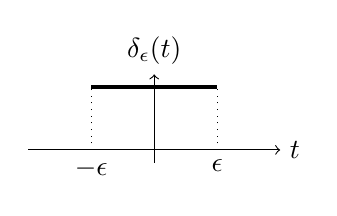
\begin{tikzpicture}[scale=0.8, baseline={(current bounding box.center)}]
      \pgfmathsetmacro{\eps}{1} % for plotting purposes, assume epsilon=1
      \pgfmathsetmacro{\hgt}{1/(\eps)}
      % Axes
      \draw[->] (-2,0) -- (2,0) node[right] {$t$};
      \draw[->] (0,-0.2) -- (0,1.2) node[above] {$\delta_{\epsilon}(t)$};
      % Plot: horizontal line over (-eps,eps) at height hgt
      \draw[line width=1.2pt] (-\eps,\hgt) -- (\eps,\hgt);
      % Dotted vertical lines showing the jump edges
      \draw[dotted] (-\eps,0) -- (-\eps,\hgt);
      \draw[dotted] (\eps,0) -- (\eps,\hgt);
      % Optionally, label the edges
      \node[below] at (-\eps,0) {$-\epsilon$};
      \node[below] at (\eps,0) {$\epsilon$};
    \end{tikzpicture}
     &
    \delta_{\epsilon}(t)=
    \begin{cases}
      \dfrac{1}{2\epsilon} & \text{if } -\epsilon < t < \epsilon, \\
      0                    & \text{otherwise.}
    \end{cases}
  \end{array}
$$
Notice that that the area under the curve is $1$:
$$\int_{-\infty}^{\infty} \delta_{\epsilon}(t)\; dt = \int_{-\epsilon}^{\epsilon} \frac{1}{2 \epsilon} \; dt = \frac{2\epsilon}2{\epsilon}  = 1$$
As $\epsilon \to 0$, the function becomes infinitely tall and thin, but the area remains $1$. The Dirac Delta Function is defined as:
$$\delta(t) = \lim_{\epsilon \to 0+} \{\delta_{\epsilon}(t)\}$$
The Dirac Delta Function has the property:
$$\delta(t) = 0 \;\; \text{for} \;\; t \neq 0 \quad \text{and} \quad \int_{-\infty}^{\infty} \delta(t) \; dt = 1$$

\end{document}